%!TEX root =  pulse_fitting_poster.tex
\begin{center}
  \begin{center} {\bf \Large \textsf {Outlook: Arrival Time Estimation}}\end{center}
\end{center}
% We demonstrated a technique that counts photons using the area of a signal portion identified with a discriminator. 
% This technique is a useful alternative to identifying the number of pulse edges using differentiation, especially when signal-to-noise ratio is small.
% \vspace{1cm}
As an extension to this technique, we use the discriminator region to bound the range of values expected for the arrival time of individual pulses in a trace containing $N$ overlapping signals. 
%
We use this bound to initialise a least-squares fit of the signal to a multi-photon model comprising of a linear superposition of $N$ single-photon models.
%
The fit returns the amplitudes and arrival times of the individual pulses.
%
\begin{figurehere}
  \begin{minipage}{0.7\linewidth}
    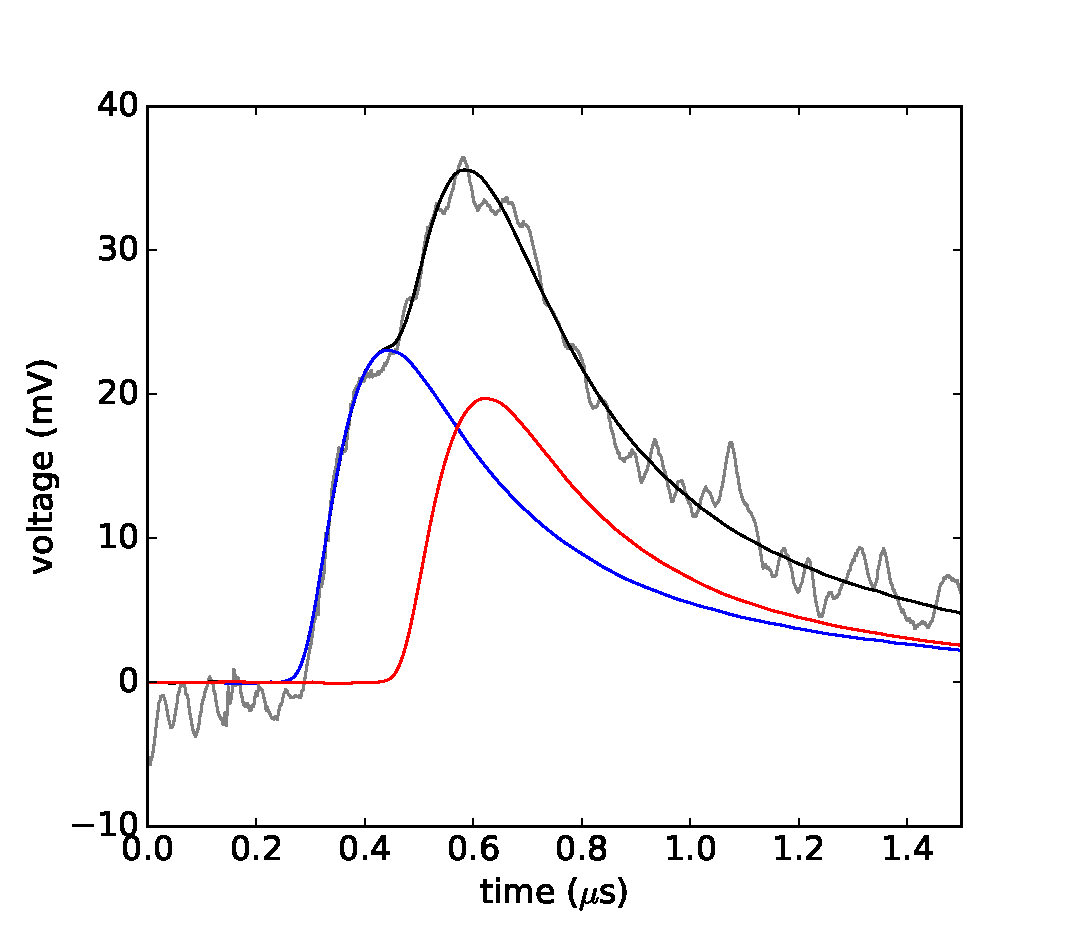
\includegraphics[width=1\linewidth]{figures/mcmc_components_170ns/mcmc_fitted_components_170ns.eps}
  \end{minipage}
  \begin{minipage}{0.3\linewidth}

    \figcaption{\label{fig:height_histo}
    Fit (black) of a 2-photon signal (grey) composed of individual single photon events (red, blue) separated by ~$\sim$170~ns, comparable to twice the rise time of a single photon pulse. 
    %
    The single photon model was obtained by averaging 10000 single photon detection events.
}
  \end{minipage}
\end{figurehere}